\section{Implementierung}
    Es handelt sich um einen Intergrationstests. Bei diesen Tests wird die Software komplett getestet, so wie sie dann im Betrieb ist.
    Aus diesem Grund, jedes Setup der Software wird Zeit in Anspruch nehmen und man soll das lieber soweit es möglich vermeiden. 
    Es gibt mehrere Möglichkeiten dies zu vermeiden:
    \begin{itemize}
        \item mehrere Tests pro Setup zu definieren und auszuführen.
        \item  die Tests die in unterschiedlichen Setups ablaufen (d.h. nicht miteinader verbunden) parallel laufen zu lassen.
    \end{itemize}

    % Um die Einarbeitungszeit in das Testframework klein zu halten, wurde entschieden das OCPPServer Testframework 
    % basierend auf ein anderes Framework, das von dem Team bereits genutzt wird. Dieses Framework wird um die neuen Funktionalitäten erweitert
    % und das restliche Verhalten soll genauso bleiben.

    Um die Lesbarkeit des Tests zu verbessern wäre es vom Vorteil, wenn die erstellte OCPPServer Testinstanz bereits ein vordefiniertes Verhalten besitzt, 
    das man ändern kann.

    Es soll auch möglich sein das vordefinierte Verhalten zu parametrieren. Dies erfordert einen Interfaces, die bestimmte Parameter der Instanz ändern kann.

    Da nur das Verhalten von dem Charging Point getestet werden soll, sollen nur die Ereignisse, die den Zustand des Charging Points abbilden, abrufbar sein.
    Zum Beispiel: geschickte Nachrichten von dem Charging Point zu dem Server, Reihenfolge der Nachrichten.

    \subsection{Achitecture des Frameworks}
    Es wurde entschieden das Framework in 7 Abstraktionsschichten aufzuteilen.
        \subsubsection{Ports}
        Ports haben die Aufgabe die Schnittstelle nach Außen aufzubauen und die Verbindungen zu .... (z.B. WebSocket Server, Datenbank)

        In dem Framework wird nur ein Port gebraucht - WebSocket Server
        \subsubsection{Adapters}
        Adapters sollen die ankommenden Events/Messages vom Port an das dazugehörige Controller zu übersetzen.

        In dem Framework wird nur einen Adapter gebraucht - OCPP16 Adapter
        \subsubsection{Controllers}
        Controllers besitzen alle Informationen die den Zustand des jeweiligen Components (Controller + Adapter + Port) abbilden.

        In dem Framework werden mehrere Controllers gebraucht:
        \begin{itemize}
            \item OCPP Controller(übernimmt die Verantwortung über die Verbindungen zu den Charging Points)
            \item User Controller(übernimmt die Verantwortung über die Nutzer der Charging Points und ihrer Berechtigungen)
            \item Transaction Controller(übernimmt die Verantwortung über die Kontroller über die Ladevorgängen)
            \item Charger Controller(übernimmt die Verantwortung über die Charging Points, die von dem Server bekannt sind und ihrer Zuständen)
            \item Payment Controller(übernimmt die Verantwortung über die Bezahlvorgang nach dem Ladevorgang)
        \end{itemize}

        Die Contoller können von dem Nutzer des Frameworks parametriert werden, um das Verhalten des Servers zu ändern.
        \subsubsection{Dispatcher}
        Dispatcher informiert alle abonnierten UseCases über das geschehene Event

        In dem Framework sind nur OCPP Events wichtig (Nachrichten und Verbindungsevent)
        \subsubsection{UseCases}
        UseCases beschreiben den Vorgang beim geschehen eines Events, das von denen abonniert wurde.
        Die vordefinierten UseCases dürfen nur die Interactor benutzen um das Verhalten zu definieren.

        In dem Framework sind die UseCases, die das vordefinierte Verhalten definieren und sie können auch entsprechend umbeschrieben werden.
        \subsubsection{Interactors}
        Eine atomare Operation im Programm(die Operation lässt sich nicht mehr sinnvoll im Rahmen der Anwendung aufgeteilen).
        Benutzt mittels "Dependency Injection" die Controller.

        In dem Framework wird nur als "Wrapper" für alle Funktionen von Controllern implementiert.
        \subsubsection{Domain}
        Definiert alle Types und Interfaces der Applications.
        Definiert die Verbindungen zwischen den Interfaces und Types, die dann in den anderen 6 Layers umgesetz werden.

    \subsection{Zugriff vom Testframework}
    \begin{itemize}
        \item OCPPPort soll nur bei der Initialisierung der Instanz parametrierbar sein (Netzwerkeinstellung)
        \item Adapters sollen nicht von der Seite des Frameworks aufrufbar sein
        \item Contollers sollen nicht von der Seite des Frameworks aufrufbar sein
        \item Dispatcher darf nur zum Abonnieren/Disabonnieren benutzt werden um das Verhalten des Charging Points beobachten zu können
        \item UseCases sollen überschreibar und erweitbar sein, falls man bestimmtes Verhalten hinzufügen möchte.
        \item Interactors sollen von der Seite des Frameworks aufrufbar sein, um die Serverinstanz parametrieren zu können.
        \item Domain beinhaltet alle Typen die in den anderen Layers benutzt werden. Aus diesem Grund sollen die Typen von der Seite des Frameworks benutzbar sein.
    \end{itemize}

    \subsection{Testbeispiel}
    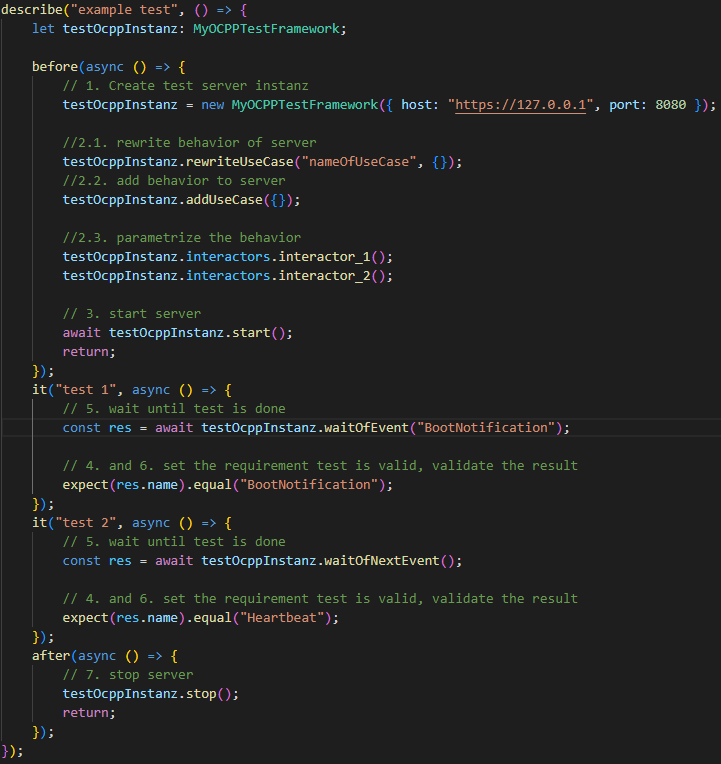
\includegraphics[width=1\textwidth,center]{Images/TestExample.png}\\[1cm]
